% Drawing 85/05-3 -- folder 85, batch 05, archive page 97 (PDF page 98).
% Transcription: figures. En haut à gauche, un grand treillis en perspective des classes de sous-groupes de $\mathfrak{S}_5$, repris de la page 95 et mis au net, dont les sommets sont $\mathfrak{A}_2 = 1$, $\mathfrak{S}_2$, $\mathbb{F}_2$, $\mathfrak{S}_2 \times \mathfrak{S}'_2 = \mathfrak{S}_2 \times \mathbb{F}_2$, $\mathbb{D}_2 = \mathbb{F}_2^{2}$, $\mathbb{Z}_4$, $\mathbb{D}_4$, $\mathfrak{S}_3$, $\mathbb{Z}_6$, $\mathbb{D}_3$, $\mathfrak{S}_3 \times \mathfrak{S}''_2$, $\mathfrak{A}_3 = \mathbb{Z}_3$, $\mathfrak{A}_4$, $\mathfrak{S}_4$, $\mathfrak{A}_5$, $\mathfrak{S}_5$, $\mathbb{D}_5$, $\mathbb{Z}_5$ ; les arêtes portent des indices ($2$, $3$, $5$), certaines en pointillé, et une bande ombrée longe le chemin de $\mathfrak{A}_3$ à $\mathfrak{A}_5$. En bas à gauche, des correspondances marquées de doubles flèches : $\mathbb{F}_2 \leftrightarrow \mathbb{Z}/4 \leftrightarrow \mathbb{D}_4 \leftrightarrow \mathfrak{S}_4 \times \mathbb{F}_2$, $\mathbb{D}_2 \leftarrow \mathfrak{A}_4 \leftrightarrow \mathfrak{S}_4$, $\mathbb{D}_3 \leftrightarrow \mathfrak{S}_3 \leftrightarrow \mathbb{D}_3 \leftrightarrow \mathfrak{S}_3 \times \mathfrak{S}''_2$, $\mathbb{D}_5 \leftrightarrow \mathbb{Z}_5$, $\mathbb{Z}_6$, avec des groupes entourés et une ligne biffée ; tout en bas, deux petits schémas : $\mathfrak{S}_3$ au-dessus de $\mathfrak{A}_3$, et un rectangle $\mathfrak{S}_2$ -- $\mathfrak{S}_3$ -- $\mathfrak{S}_3 \times \mathfrak{S}'_3$, $\mathfrak{A}_3$ -- $\mathbb{D}_3$
% Kind: perspective lattice of the classes of subgroups of S5, correspondences, two small schemes. Method 2 (schematic redraw from the facsimile). Status: partial.
% Notes: Upper left: the perspective lattice, vertices labelled after the transcription and placed on the facsimile, edges drawn between node centres with the indices 2, 3, 5 that can be read; the shaded band from A3 to A5 is drawn as two curves (shading left out); dotted strokes partly left out. Lower left: the correspondences with double arrows, circled groups circled, the struck line drawn grey and schematised (a scribbled group near S3 x S2'' is left out). Bottom: S3 over A3, and the rectangle S2 -- S3 -- S3 x S3', A3 -- D3. A small arrow with S3 at bottom left, not in the transcription, is drawn. The text on the right (counts of classes, normalisers) is left out. Issue 128 pass: the lattice edges were already drawn between the same node points; the few line ends that nearly met were merged into one computed vertex, and the labels set at \small. Still differs, and not re-read in this pass: the node positions and the uncertain vertex readings above, the dotted strokes partly left out, the shading. Redrawn 2026-11-09 (issue 128): to check again.
% Coordinates: 1 unit = 1 mm = 1/100 of the crop width (bbox in page fractions: [0.05, 0.05, 0.95, 0.86]).
% Redrawn by Claude (claude-opus-5-5), issue #73, 2026-11-09; not checked by a human; not compiled (no TeX in the session).
% Rights: reproduces part of the work -- behind RENDER_TRANSCRIPTS, never published by itself.
\documentclass[tikz,border=3pt]{standalone}
\usepackage{amsmath,amssymb}
\usetikzlibrary{patterns,arrows.meta}
\tikzset{pencil/.style={black!45}, struck/.style={black!35}, mark/.style={circle,draw,inner sep=1.3pt}, pt/.style={circle,fill,inner sep=0.9pt}, opt/.style={circle,draw,fill=white,inner sep=1.1pt}}
\begin{document}
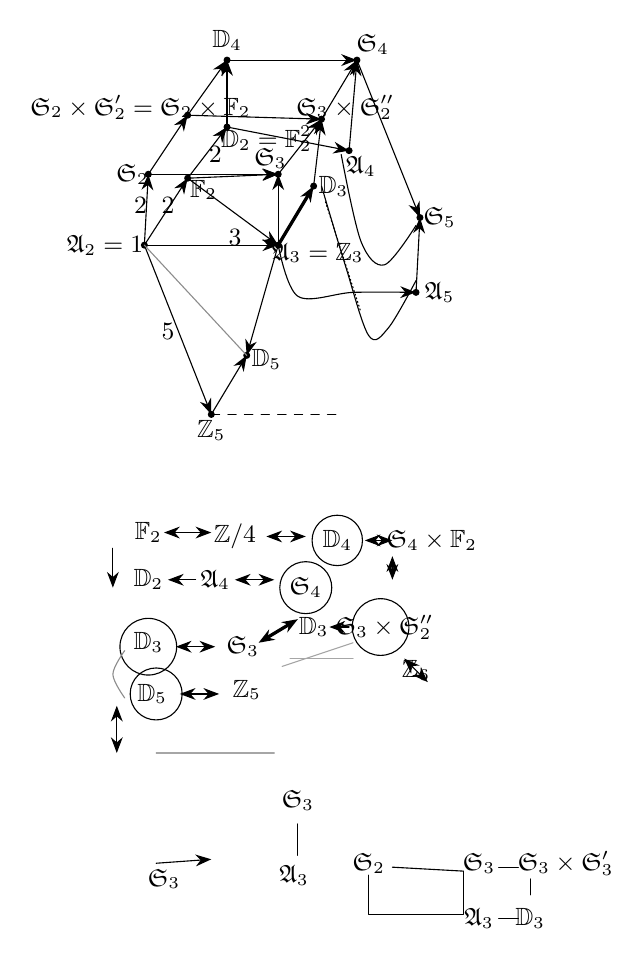
\begin{tikzpicture}[x=1mm,y=1mm,line cap=round,line join=round,font=\scriptsize]
\node[pt] at (22,-10) {};
\node[pt] at (38.5,-10) {};
\node[pt] at (17,-17) {};
\node[pt] at (22,-18.5) {};
\node[pt] at (34,-17.5) {};
\node[pt] at (37.5,-21.5) {};
\node[pt] at (12,-24.5) {};
\node[pt] at (28.5,-24.5) {};
\node[pt] at (17,-25) {};
\node[pt] at (33,-26) {};
\node[pt] at (46.5,-30) {};
\node[pt] at (11.5,-33.5) {};
\node[pt] at (28.5,-33.5) {};
\node[pt] at (46,-39.5) {};
\node[pt] at (24.5,-47.5) {};
\node[pt] at (20,-55) {};
\node[inner sep=1pt] at (22,-7.5) {\small $\mathbb{D}_4$};
\node[inner sep=1pt] at (40.5,-8) {\small $\mathfrak{S}_4$};
\node[inner sep=1pt] at (11,-16) {\small $\mathfrak{S}_2\times\mathfrak{S}'_2=\mathfrak{S}_2\times\mathbb{F}_2$};
\node[inner sep=1pt] at (27,-20) {\small $\mathbb{D}_2=\mathbb{F}_2^2$};
\node[inner sep=1pt] at (37,-16) {\small $\mathfrak{S}_3\times\mathfrak{S}''_2$};
\node[inner sep=1pt] at (39,-23.5) {\small $\mathfrak{A}_4$};
\node[inner sep=1pt] at (10,-24.5) {\small $\mathfrak{S}_2$};
\node[inner sep=1pt] at (27.5,-22.5) {\small $\mathfrak{S}_3$};
\node[inner sep=1pt] at (19,-26.5) {\small $\mathbb{F}_2$};
\node[inner sep=1pt] at (35.5,-26) {\small $\mathbb{D}_3$};
\node[inner sep=1pt] at (49,-30) {\small $\mathfrak{S}_5$};
\node[inner sep=1pt] at (6.5,-33.5) {\small $\mathfrak{A}_2=1$};
\node[inner sep=1pt] at (33.5,-34.5) {\small $\mathfrak{A}_3=\mathbb{Z}_3$};
\node[inner sep=1pt] at (49,-39.5) {\small $\mathfrak{A}_5$};
\node[inner sep=1pt] at (27,-48) {\small $\mathbb{D}_5$};
\node[inner sep=1pt] at (20,-57) {\small $\mathbb{Z}_5$};
\draw[-{Stealth[length=2mm]}] (11.5,-33.5) -- (12,-24.5);
\draw[-{Stealth[length=2mm]}] (11.5,-33.5) -- (17,-25);
\draw[-{Stealth[length=2mm]}] (11.5,-33.5) -- (28.5,-33.5);
\draw[-{Stealth[length=2mm]}] (12,-24.5) -- (28.5,-24.5);
\draw[-{Stealth[length=2mm]}] (17,-25) -- (28.5,-24.5);
\draw[-{Stealth[length=2mm]}] (12,-24.5) -- (17,-17);
\draw[-{Stealth[length=2mm]}] (17,-25) -- (22,-18.5);
\draw[-{Stealth[length=2mm]}] (17,-17) -- (22,-10);
\draw[-{Stealth[length=2mm]}] (22,-18.5) -- (22,-10);
\draw[-{Stealth[length=2mm]}] (22,-10) -- (38.5,-10);
\draw[-{Stealth[length=2mm]}] (17,-17) -- (34,-17.5);
\draw[-{Stealth[length=2mm]}] (28.5,-24.5) -- (34,-17.5);
\draw[-{Stealth[length=2mm]}] (34,-17.5) -- (38.5,-10);
\draw[-{Stealth[length=2mm]}] (37.5,-21.5) -- (38.5,-10);
\draw[-{Stealth[length=2mm]}] (22,-18.5) -- (37.5,-21.5);
\draw[-{Stealth[length=2mm]}] (38.5,-10) -- (46.5,-30);
\draw[-{Stealth[length=2mm]}] (46,-39.5) -- (46.5,-30);
\draw[-{Stealth[length=2mm]}] (28.5,-33.5) -- (28.5,-24.5);
\draw[very thick,-{Stealth[length=2mm]}] (28.5,-33.5) -- (33,-26);
\draw[-{Stealth[length=2mm]}] (33,-26) -- (34,-17.5);
\draw[-{Stealth[length=2mm]}] (17,-25) -- (28.5,-33.5);
\draw[-{Stealth[length=2mm]}] (11.5,-33.5) -- (20,-55);
\draw[-{Stealth[length=2mm]}] (20,-55) -- (24.5,-47.5);
\draw[-{Stealth[length=2mm]}] (28.5,-33.5) -- (24.5,-47.5);
\draw[pencil] (11.5,-33.5) -- (24.5,-47.5);
\draw[dashed] (20,-55) -- (36,-55);
\draw[-{Stealth[length=2mm]}] plot[smooth, tension=0.55] coordinates {(28.5,-33.5) (31,-40) (38,-39.5) (46,-39.5)};
\draw plot[smooth, tension=0.55] coordinates {(34,-26) (37,-36) (40,-45) (42.5,-44) (46,-38)};
\draw plot[smooth, tension=0.55] coordinates {(36.5,-22) (39,-33) (42,-36) (46,-31)};
\draw[densely dotted] (34.5,-28) -- (39,-42);
\node[inner sep=1pt] at (11,-28.5) {\small $2$};
\node[inner sep=1pt] at (14.5,-28.5) {\small $2$};
\node[inner sep=1pt] at (20.5,-22) {\small $2$};
\node[inner sep=1pt] at (23,-32.5) {\small $3$};
\node[inner sep=1pt] at (14.5,-44.5) {\small $5$};
\node[inner sep=1pt] at (12,-70) {\small $\mathbb{F}_2$};
\draw[{Stealth[length=2mm]}-{Stealth[length=2mm]}] (14,-70) -- (20,-70);
\node[inner sep=1pt] at (23,-70.5) {\small $\mathbb{Z}/4$};
\draw[{Stealth[length=2mm]}-{Stealth[length=2mm]}] (27,-70.5) -- (32,-70.5);
\node[inner sep=1pt] at (36,-71) {\small $\mathbb{D}_4$};
\draw (36,-71) circle[radius=3.2];
\draw[{Stealth[length=2mm]}-{Stealth[length=2mm]}] (39.5,-71) -- (43,-71);
\node[inner sep=1pt] at (48,-71) {\small $\mathfrak{S}_4\times\mathbb{F}_2$};
\draw[{Stealth[length=2mm]}-{Stealth[length=2mm]}] (43,-73) -- (43,-76);
\node[inner sep=1pt] at (12,-76) {\small $\mathbb{D}_2$};
\draw[{Stealth[length=2mm]}-] (14.5,-76) -- (18,-76);
\node[inner sep=1pt] at (20.5,-76) {\small $\mathfrak{A}_4$};
\draw[{Stealth[length=2mm]}-{Stealth[length=2mm]}] (23,-76) -- (28,-76);
\node[inner sep=1pt] at (32,-77) {\small $\mathfrak{S}_4$};
\draw (32,-77) circle[radius=3.3];
\draw[-{Stealth[length=2mm]}] (7.5,-72) -- (7.5,-77);
\node[inner sep=1pt] at (12,-84) {\small $\mathbb{D}_3$};
\draw (12,-84.5) circle[radius=3.6];
\draw[{Stealth[length=2mm]}-{Stealth[length=2mm]}] (15.5,-84.5) -- (20.5,-84.5);
\node[inner sep=1pt] at (24,-84.5) {\small $\mathfrak{S}_3$};
\draw[{Stealth[length=2mm]}-{Stealth[length=2mm]},very thick] (26,-84) -- (31,-81);
\node[inner sep=1pt] at (33,-82) {\small $\mathbb{D}_3$};
\draw[{Stealth[length=2mm]}-] (35,-82) -- (37.5,-82);
\node[inner sep=1pt] at (42,-82) {\small $\mathfrak{S}_3\times\mathfrak{S}''_2$};
\draw (41.5,-82) circle[radius=3.6];
\node[inner sep=1pt] at (46,-87.5) {\small $\mathbb{Z}_6$};
\draw[{Stealth[length=2mm]}-{Stealth[length=2mm]}] (44.5,-86) -- (47.5,-89);
\node[inner sep=1pt] at (12.5,-90.5) {\small $\mathbb{D}_5$};
\draw (13,-90.5) circle[radius=3.3];
\draw[{Stealth[length=2mm]}-{Stealth[length=2mm]}] (16,-90.5) -- (21,-90.5);
\node[inner sep=1pt] at (24.5,-90) {\small $\mathbb{Z}_5$};
\draw[pencil] plot[smooth, tension=0.55] coordinates {(9,-85) (7.5,-88) (9,-91)};
\draw[{Stealth[length=2mm]}-{Stealth[length=2mm]}] (8,-92) -- (8,-98);
\draw[struck] (29,-87) -- (38,-84);
\draw[struck] (30,-86) -- (38,-86);
\draw[struck] (13,-98) -- (28,-98);
\node[inner sep=1pt] at (31,-104) {\small $\mathfrak{S}_3$};
\draw (31,-107) -- (31,-111);
\node[inner sep=1pt] at (30.5,-113.5) {\small $\mathfrak{A}_3$};
\node[inner sep=1pt] at (40,-112) {\small $\mathfrak{S}_2$};
\draw (43,-112.5) -- (52,-113);
\node[inner sep=1pt] at (54,-112) {\small $\mathfrak{S}_3$};
\draw (56.5,-112.5) -- (59,-112.5);
\node[inner sep=1pt] at (65,-112) {\small $\mathfrak{S}_3\times\mathfrak{S}'_3$};
\draw (60.5,-114) -- (60.5,-116);
\draw (40,-113.5) -- (40,-118.5) -- (52,-118.5) -- (52,-113);
\node[inner sep=1pt] at (54,-119) {\small $\mathfrak{A}_3$};
\draw (56.5,-119) -- (59,-119);
\node[inner sep=1pt] at (60.5,-119) {\small $\mathbb{D}_3$};
\draw[-{Stealth[length=2mm]}] (13,-112) -- (20,-111.5);
\node[inner sep=1pt] at (14,-114) {\small $\mathfrak{S}_3$};
\end{tikzpicture}
\end{document}
